% Informe escrito del trabajo de investigación MA-1006 (I Ciclo 2026).
% Compilar: ./build.sh   (pdflatex + bibtex + pdflatex x2)
\documentclass[conference]{IEEEtran}
\IEEEoverridecommandlockouts
\usepackage[utf8]{inputenc}
\usepackage[T1]{fontenc}
\usepackage{cite}
\usepackage{amsmath,amssymb,amsfonts}
\usepackage{graphicx}
\usepackage{xcolor}
\usepackage[spanish, es-nosectiondot, es-noshorthands, es-tabla]{babel}
% El espaciado antes de % lo ponemos a mano (\,\%); sin esto, la redefinición
% de \% de babel-spanish choca con el pegamento de modo matemático.
\spanishplainpercent
\usepackage{url}
\usepackage{booktabs}
\usepackage{listings}

\graphicspath{{../code/figures/}}

\newcommand{\R}{\mathbb{R}}
\newcommand{\E}{\mathbb{E}}
\newcommand{\norm}[1]{\left\lVert #1 \right\rVert}

\renewcommand{\IEEEkeywordsname}{Palabras clave}
\renewcommand{\lstlistingname}{Listado}

\lstset{
  language=Python,
  basicstyle=\ttfamily\footnotesize,
  keywordstyle=\bfseries,
  commentstyle=\itshape,
  showstringspaces=false,
  frame=single,
  framerule=0.4pt,
  aboveskip=6pt,
  belowskip=6pt,
  xleftmargin=4pt,
  xrightmargin=4pt,
}

\begin{document}

% Portada independiente: una columna, sin número de página. El artículo
% propiamente dicho reinicia la numeración en 1 después de esta página.
\onecolumn
\thispagestyle{empty}
\begin{center}
    \vspace*{2.5cm}

    {\Large \textsc{Universidad de Costa Rica}}\\[0.6em]
    {\large Facultad de Ciencias}\\[0.4em]
    {\large Escuela de Matemática}\\[0.4em]
    {\large MA-1006 Introducción al Análisis Numérico, Grupo 01}

    \vfill

    {\large Trabajo de investigación}\\[1.2em]
    {\LARGE\bfseries Implementación de técnicas de descenso\\[0.35em]
    de gradiente estocástico y variantes}

    \vfill

    {\large Ariel Arévalo Alvarado}\\[0.4em]
    {\large Carné B50562}\\[2em]
    {\large Profesor: Óscar Salas Huertas}

    \vfill

    {\large I Ciclo 2026}\\[0.4em]
    {\large 5 de julio de 2026}

    \vspace*{1.5cm}
\end{center}
\twocolumn
\setcounter{page}{1}


\title{Implementación de técnicas de descenso de gradiente estocástico y variantes\\
\thanks{Trabajo de investigación del curso MA-1006 Introducción al Análisis Numérico, Grupo 01, I Ciclo 2026, Universidad de Costa Rica. Profesor: Óscar Salas Huertas.}
}

\author{
\IEEEauthorblockN{Ariel Arévalo Alvarado}
\IEEEauthorblockA{\textit{Escuela de Ciencias de la Computación e Informática} \\
\textit{Universidad de Costa Rica}\\
San José, Costa Rica \\
ariel.arevalo@ucr.ac.cr \\
Carné B50562}
}

\IEEEaftertitletext{\begin{center}\itshape 5 de julio de 2026\end{center}}
\maketitle

\begin{abstract}
El entrenamiento de un modelo de aprendizaje automático consiste en minimizar el riesgo empírico, un promedio de pérdidas sobre los $n$ datos. A gran escala solo resultan viables los métodos iterativos de primer orden, y la forma de suma del objetivo permite abaratar cada iteración estimando el gradiente con una muestra. Se implementan en NumPy, como funciones de actualización puras de menos de diez líneas, el descenso de gradiente (GD), su versión estocástica (SGD) con mini-lotes, el criterio de parada temprana y la variante de Momentum. Los métodos se comparan sobre dos superficies de prueba clásicas, una cuadrática mal condicionada y la función de Rosenbrock, y sobre una regresión logística regularizada con datos reales (UCI Banknote Authentication, $n = 1372$), contabilizando el costo en épocas para que la comparación sea por unidad de cómputo. Los resultados reproducen la teoría: SGD domina a GD por época desde la primera pasada, el tamaño del lote regula la varianza del estimador, la parada temprana actúa como regularización sin costo adicional, y Momentum acelera justo donde la geometría es adversa, con una mejora de cuatro órdenes de magnitud sobre GD en Rosenbrock.
\end{abstract}

\begin{IEEEkeywords}
análisis numérico, optimización, descenso de gradiente estocástico, mini-lotes, Momentum, parada temprana, regresión logística
\end{IEEEkeywords}

\section{Introducción}\label{sec:intro}

Detrás de todo modelo que ``aprende'' hay un problema de optimización numérica. Ajustar una regresión, un clasificador o un modelo de lenguaje consiste en elegir un vector de parámetros $\theta$ que minimice el riesgo empírico,
\begin{equation}
  f(\theta) = \frac{1}{n}\sum_{i=1}^{n} \ell_i(\theta),
  \label{eq:erm}
\end{equation}
donde $\ell_i$ mide qué tan mal predice $\theta$ el dato $i$. Esta forma de promedio finito encierra a la vez el problema y su solución. El problema: el gradiente exacto, $\nabla f = \frac{1}{n}\sum_i \nabla\ell_i$, también es una suma, y evaluarlo cuesta una pasada completa por los $n$ datos. La solución: por ser un promedio, puede estimarse con una muestra, a una fracción del costo.

En el régimen moderno, tanto $n$ como la dimensión $d$ de $\theta$ alcanzan los miles de millones, y eso descarta la maquinaria clásica de orden superior: el método de Newton exige formar la matriz Hessiana y resolver un sistema con ella, con costo $O(nd^2 + d^3)$ por iteración~\cite{bottou2018}. Sobreviven los métodos de primer orden, que solo consultan el gradiente. Su lógica es la misma que recorre todo el curso de análisis numérico: construir un modelo local con el polinomio de Taylor, dar un paso según ese modelo y repetir.

Este trabajo implementa y estudia esa familia. Se deriva el descenso de gradiente (GD) junto con su condición de estabilidad, se introduce la versión estocástica (SGD) y su generalización por mini-lotes, se presenta el criterio práctico de parada temprana y se analiza la variante de Momentum de Polyak. Todos los métodos se implementan en NumPy como funciones de actualización puras de menos de diez líneas, se verifican sobre superficies de prueba con mínimo conocido y se comparan sobre una regresión logística con datos reales, bajo una contabilidad de costo en épocas que hace las comparaciones justas.

El resto del documento se organiza así. La Sección~\ref{sec:preliminares} fija la notación y la lectura geométrica del problema. La Sección~\ref{sec:gd} deriva GD desde el polinomio de Taylor y analiza su convergencia, su estabilidad y su costo. Las Secciones~\ref{sec:sgd} y~\ref{sec:minilotes} introducen el estimador estocástico del gradiente, el mini-lote y la parada temprana. La Sección~\ref{sec:momentum} presenta Momentum. La Sección~\ref{sec:impl} describe la implementación y la Sección~\ref{sec:exp} los experimentos y resultados. La Sección~\ref{sec:concl} concluye.

\section{Preliminares}\label{sec:preliminares}

\subsection{Notación y unidades de costo}

A lo largo del documento, $\theta \in \R^d$ es el vector de parámetros del modelo, $\ell_i : \R^d \to \R$ es la pérdida asociada al dato $i$, y $f$ es el riesgo empírico~\eqref{eq:erm}. El gradiente $\nabla f(\theta)$ apunta en la dirección de mayor crecimiento local de $f$, el escalar $\alpha > 0$ es la tasa de aprendizaje (el tamaño de paso) y $k$ indexa las iteraciones.

Conviene distinguir dos unidades de cuenta que el resto del trabajo usa sin descanso. Una \emph{iteración} es una actualización del vector $\theta$. Una \emph{época} es una pasada completa por los $n$ datos, es decir, $n$ evaluaciones de gradientes individuales $\nabla\ell_i$. La relación entre ambas depende del método: GD consume una época entera por iteración, mientras que los métodos estocásticos realizan muchas iteraciones por época. Por eso, en este trabajo las comparaciones entre métodos se hacen siempre por épocas, que miden trabajo computacional, y nunca por iteraciones, que no cuestan lo mismo entre métodos.

\subsection{El paisaje de pérdida}

La lectura geométrica que ancla todo lo demás: cada punto $\theta$ del espacio de parámetros es un modelo candidato, y $f$ le asigna una altura. El riesgo empírico define así una superficie sobre $\R^d$, y entrenar es descender por ella hasta el punto más bajo.

Con $d = 2$ la superficie se puede dibujar. Para una regresión lineal por mínimos cuadrados, $y \approx \theta_0 + \theta_1 x$, la pérdida es cuadrática en $\theta$: la superficie es un paraboloide convexo con un único mínimo, dado en forma cerrada por las ecuaciones normales. Ese caso, visualizable y con respuesta exacta conocida, sirve de banco de calibración en las Secciones~\ref{sec:gd} y~\ref{sec:sgd}. En un problema real, en cambio, $d$ es enorme: no se puede ver la superficie ni resolver en forma cerrada, y lo único disponible es la pendiente local $\nabla f(\theta)$ en el punto actual. Entrenar es descender por una superficie invisible sintiendo únicamente la pendiente bajo los pies. Todos los métodos de este trabajo son estrategias para ese descenso.

\section{Del polinomio de Taylor al descenso de gradiente}\label{sec:gd}

\subsection{Derivación}

El método sale de la herramienta central del curso: el polinomio de Taylor. Cerca de un punto $\theta$, el modelo local de primer orden de $f$ es
\begin{equation}
  f(\theta + \Delta) = f(\theta) + \nabla f(\theta)^{\mathsf{T}}\Delta + O\bigl(\norm{\Delta}^2\bigr).
  \label{eq:taylor}
\end{equation}
Si se elige el desplazamiento $\Delta = -\alpha\,\nabla f(\theta)$, el término lineal se vuelve $-\alpha\norm{\nabla f(\theta)}^2 \leq 0$: mientras el gradiente no sea nulo, el modelo local predice descenso. Es además la mejor elección posible: entre todos los $\Delta$ de norma fija, el producto $\nabla f^{\mathsf{T}}\Delta$ se minimiza cuando $\Delta$ es antiparalelo a $\nabla f$, por la desigualdad de Cauchy-Schwarz. De ahí el método completo,
\begin{equation}
  \theta_{k+1} = \theta_k - \alpha\,\nabla f(\theta_k).
  \label{eq:gd}
\end{equation}
Tiene una sola perilla, $\alpha$, y es la más delicada de todas, porque $\alpha$ controla exactamente el término $O(\norm{\Delta}^2)$ que el modelo local ignora. Con $\alpha$ pequeño el modelo es fiel: el descenso es seguro pero lento. Con $\alpha$ grande, el término ignorado puede superar al lineal y hacer subir a $f$.

\subsection{Convergencia y estabilidad en cuadráticas}

Para una $f$ cuadrática con Hessiana $H$ simétrica definida positiva y mínimo $\theta^*$, la iteración~\eqref{eq:gd} da una recurrencia exacta para el error:
\begin{equation}
  \theta_{k+1} - \theta^* = (I - \alpha H)\,(\theta_k - \theta^*).
  \label{eq:recurrencia}
\end{equation}
En la base de vectores propios de $H$, la componente del error asociada al valor propio $\lambda_i$ se multiplica por $(1 - \alpha\lambda_i)$ en cada iteración. El método converge si y solo si $|1 - \alpha\lambda_i| < 1$ en toda dirección, es decir,
\begin{equation}
  0 < \alpha < \frac{2}{\lambda_{\max}}.
  \label{eq:estabilidad}
\end{equation}
Con la tasa óptima $\alpha^* = 2/(\lambda_{\max} + \lambda_{\min})$, el error se contrae por el factor $(\kappa - 1)/(\kappa + 1)$ por iteración, donde $\kappa = \lambda_{\max}/\lambda_{\min}$ es el número de condición de $H$. La velocidad de GD la gobierna la geometría del problema, no solo su tamaño.

El fenómeno se observa con precisión sobre el problema sintético de mínimos cuadrados de la Sección~\ref{sec:impl} ($n = 80$ datos, dos parámetros), cuya Hessiana tiene valores propios $1.454$ y $0.958$, de modo que el límite~\eqref{eq:estabilidad} es $\alpha < 1.375$. Partiendo del mismo punto: con $\alpha = 0.015$ el método avanza tan poco que tras 80 iteraciones sigue en la ladera del tazón ($f \approx 0.614$). Con $\alpha = 0.8$ baja directo al fondo ($f \approx 0.321$, el error irreducible impuesto por el ruido de los datos). Con $\alpha = 1.25$, el factor en la dirección más rígida es $1 - 1.25 \cdot 1.454 \approx -0.82$: negativo, por lo que la trayectoria alterna de lado, pero de magnitud menor que uno, por lo que aun así converge. Con $\alpha = 1.381$ ese factor vale $\approx -1.008$: cada rebote sube un poco más que el anterior hasta escapar del tazón. Entre converger y explotar hay menos de una centésima de diferencia en $\alpha$.

\subsection{Las dos debilidades}

La primera es el costo. Por la forma de suma de~\eqref{eq:erm}, cada iteración exacta de~\eqref{eq:gd} recorre los $n$ datos: $O(nd)$ operaciones, una época entera por iteración. Cuando $n$ se cuenta en miles de millones, una sola actualización de $\theta$ es prohibitiva. Romper ese acople entre el trabajo por iteración y el tamaño de los datos es el tema de la Sección~\ref{sec:sgd}.

La segunda es la geometría. Cuando $\kappa$ es grande, el paisaje es un valle angosto, el factor $(\kappa-1)/(\kappa+1)$ se acerca a uno y la trayectoria zigzaguea de pared a pared en lugar de avanzar por el fondo. Con $\kappa = 25$, el factor óptimo es $24/26 \approx 0.923$: apenas $7.7\,\%$ de reducción del error por iteración (Fig.~\ref{fig:ravine}, Sección~\ref{sec:exp}). Reparar esa geometría es el tema de la Sección~\ref{sec:momentum}.

\section{Descenso de gradiente estocástico}\label{sec:sgd}

\subsection{El estimador insesgado}

La salida al problema del costo está en la forma de promedio de~\eqref{eq:erm}. Si el índice $i$ se sortea uniformemente en $\{1, \dots, n\}$, el gradiente de un solo dato es un estimador insesgado del gradiente completo:
\begin{equation}
  \E\bigl[\nabla\ell_i(\theta)\bigr] = \frac{1}{n}\sum_{j=1}^{n} \nabla\ell_j(\theta) = \nabla f(\theta).
  \label{eq:insesgado}
\end{equation}
Barato no significa apuntar mal: significa apuntar bien en promedio, con ruido. El descenso de gradiente estocástico es la misma actualización~\eqref{eq:gd} alimentada con ese estimador,
\begin{equation}
  \theta_{k+1} = \theta_k - \alpha\,\nabla\ell_{i_k}(\theta_k),
  \label{eq:sgd}
\end{equation}
con $i_k$ sorteado en cada iteración. La iteración cuesta $O(d)$: $n$ veces menos que la de GD.

\subsection{El precio: varianza}

Lo que se paga es varianza, y no desaparece cerca del mínimo. Con tasa $\alpha$ fija, el iterado no converge a un punto: termina orbitando en una nube alrededor del óptimo cuyo radio es proporcional a $\alpha$. El resultado clásico de Robbins y Monro~\cite{robbins1951} da la salida teórica: si la tasa decrece cumpliendo $\sum_k \alpha_k = \infty$ y $\sum_k \alpha_k^2 < \infty$, el método converge al óptimo a pesar del ruido. En la práctica se suele preferir una tasa fija por tramos, que se reduce manualmente, aceptando el piso de ruido a cambio de velocidad.

\subsection{La comparación honesta}

Una iteración de GD y una de SGD no cuestan lo mismo, así que compararlos por iteraciones es engañoso. La comparación justa es por evaluaciones de gradiente o, equivalentemente, por épocas: mismo cómputo total gastado. GD consume una época entera por iteración, de modo que un presupuesto de 12 épocas se traduce en 12 iteraciones. SGD, sobre el problema sintético con $n = 80$, realiza 80 iteraciones por época, de modo que el mismo presupuesto se traduce en 960 iteraciones. En ese experimento, con $\alpha = 0.8$ para GD y $\alpha = 0.05$ para SGD, SGD ya ha reducido la mayor parte de la pérdida antes de completar su primera pasada por los datos, cuando GD apenas ha realizado su primera actualización. Ese es el trato central del método: se cambia precisión por iteración a cambio de número de iteraciones, y a gran escala el trato gana.

\section{Mini-lotes y parada temprana}\label{sec:minilotes}

\subsection{El estimador de mini-lote}

Un dato y todos los datos son los extremos de un continuo. El punto intermedio es el mini-lote: se sortea un subconjunto $B \subset \{1, \dots, n\}$ y se promedian sus gradientes,
\begin{equation}
  g = \nabla f_B(\theta) = \frac{1}{|B|}\sum_{i \in B} \nabla\ell_i(\theta),
  \label{eq:minibatch}
\end{equation}
donde $|B|$ es el tamaño del lote, que va desde $|B| = 1$ (el SGD de la sección anterior) hasta $|B| = n$ (GD exacto). La actualización es de nuevo la regla~\eqref{eq:gd} con $g$ en lugar del gradiente exacto. Del promedio se desprenden tres propiedades:
\begin{itemize}
  \item \emph{Sigue siendo insesgado.} Promediar no cambia la esperanza: el argumento de~\eqref{eq:insesgado} sobrevive intacto para cualquier $|B|$.
  \item \emph{El ruido decae con el lote.} La varianza del promedio de $|B|$ muestras aproximadamente independientes es $1/|B|$ veces la de una sola: cuadruplicar el lote reduce la desviación del ruido a la mitad.
  \item \emph{El costo por iteración crece.} Cada iteración cuesta $O(|B|\,d)$, y una época equivale a $n/|B|$ iteraciones. El costo por época es el mismo $O(nd)$ de siempre: el lote solo decide si la época se gasta en muchas iteraciones ruidosas o en pocas iteraciones limpias.
\end{itemize}

Con eso, $|B|$ se vuelve una perilla de diseño. En la práctica se elige tan grande como quepa en la memoria del acelerador, porque la ganancia marginal en varianza se aplana mientras que el número de actualizaciones por época sí se pierde. Un estimador con menos varianza tolera además pasos más largos: en los experimentos de la Sección~\ref{sec:exp}, el lote de 16 corre con una tasa cuatro veces mayor que el lote de 1.

\subsection{Parada temprana}

La segunda decisión práctica es cuándo detenerse. En un modelo con capacidad de sobra, entrenar de más memoriza el ruido: el error de entrenamiento sigue bajando indefinidamente, mientras que el error sobre datos no vistos baja, toca un mínimo y vuelve a subir. El criterio operativo es monitorear el error de validación y detenerse en su mínimo (Fig.~\ref{fig:early}, Sección~\ref{sec:exp}).

No se trata de una heurística improvisada sino de regularización~\cite{prechelt1998}. En el caso cuadrático puede demostrarse que $k$ iteraciones de GD desde el origen equivalen a resolver el problema con una penalización $\ell_2$ cuyo peso efectivo decrece al crecer $k$: detenerse antes equivale a regularizar más. La lectura cualitativa es que GD recorre primero las direcciones de curvatura alta, donde vive la señal robusta de los datos, y solo tarde las de curvatura baja, donde vive el sobreajuste. Detenerse a tiempo captura la señal sin el ruido, y no cuesta nada.

\section{Momentum}\label{sec:momentum}

GD es un método sin memoria: la dirección de cada iteración depende únicamente del gradiente actual. En un valle angosto, eso lo condena al zigzag de la Sección~\ref{sec:gd}. El remedio de Polyak~\cite{polyak1964}, conocido como el método de la bola pesada, consiste en recordar: se acumula una velocidad que promedia los gradientes recientes,
\begin{align}
  v_{k+1} &= \beta\, v_k + g_k, \label{eq:momentum-v}\\
  \theta_{k+1} &= \theta_k - \alpha\, v_{k+1}, \label{eq:momentum-theta}
\end{align}
donde $g_k$ es el gradiente en la iteración $k$ (exacto o muestreado) y $\beta \in [0, 1)$ regula cuánta memoria se conserva. Con $\beta = 0$ se recupera exactamente GD.

La velocidad $v$ es una media exponencial de los gradientes recientes, con memoria efectiva de unas $1/(1-\beta)$ iteraciones (unas diez con $\beta = 0.9$), y eso produce dos efectos complementarios. En la dirección transversal del valle, los gradientes alternan de signo entre iteraciones consecutivas y se cancelan dentro de la suma: el zigzag se amortigua. En la dirección larga del valle, apuntan siempre igual y se componen: la velocidad crece hacia $g/(1-\beta)$, de modo que con $\beta = 0.9$ el avance por iteración llega a ser hasta diez veces el de GD con la misma $\alpha$. El costo adicional es casi nulo: la misma única evaluación de gradiente por iteración, un vector de estado extra y dos líneas más de código.

La ganancia también se cuantifica. Con $\alpha$ y $\beta$ óptimos sobre una cuadrática, el factor de contracción del error pasa de $(\kappa-1)/(\kappa+1)$ a $(\sqrt{\kappa}-1)/(\sqrt{\kappa}+1)$: la dependencia baja de $\kappa$ a $\sqrt{\kappa}$. Para el valle con $\kappa = 25$ de la Sección~\ref{sec:exp}, el factor mejora de $0.923$ a $0.667$, es decir, de reducir el error un $7.7\,\%$ por iteración a reducirlo un $33\,\%$. La honestidad correspondiente: demasiada memoria se pasa de largo en las curvas del paisaje. $\beta$ es una perilla de amortiguamiento, y $0.9$ es un valor típico, no una constante universal.

Momentum es hoy una pieza central de los optimizadores por defecto en aprendizaje automático; un panorama de la familia completa de variantes puede consultarse en~\cite{ruder2016}.

\section{Implementación}\label{sec:impl}

El código de este trabajo es un paquete de NumPy con cuatro módulos: reglas de actualización, problemas de prueba, un ejecutor de experimentos y la generación de figuras.

\subsection{Reglas de actualización puras}

En \texttt{optimizers.py}, cada optimizador es un par de funciones $(\mathit{init}, \mathit{step})$: $\mathit{init}$ crea el estado inicial y $\mathit{step}$ recibe el punto actual, el gradiente y el estado, y devuelve el punto y el estado siguientes, sin efectos secundarios. GD no tiene estado; Momentum guarda la velocidad. Cada regla ocupa menos de diez líneas y aparece en el Listado~\ref{lst:steps} exactamente como se entrega.

\begin{lstlisting}[float=t, caption={Las reglas de actualización \eqref{eq:gd} y \eqref{eq:momentum-v}--\eqref{eq:momentum-theta} en \texttt{optimizers.py}.}, label={lst:steps}]
def gd_step(theta, g, state, lr=0.01):
    theta = theta - lr * g
    return theta, state

def momentum_step(theta, g, v, lr=0.01, beta=0.9):
    v = beta * v + g
    theta = theta - lr * v
    return theta, v
\end{lstlisting}

Un detalle de diseño refleja la teoría: SGD no existe como función aparte. La regla~\eqref{eq:gd} no cambia entre las Secciones~\ref{sec:gd} y~\ref{sec:minilotes}; lo que cambia es el origen de $g$. El módulo de problemas produce el gradiente exacto o el estimador de mini-lote~\eqref{eq:minibatch}, y ambos alimentan la misma \texttt{gd\_step}.

\subsection{Problemas y contabilidad}

\texttt{problems.py} implementa las superficies del estudio: la cuadrática mal condicionada $f(x,y) = \frac{1}{2}(x^2 + 25y^2)$, la función de Rosenbrock, el problema sintético de mínimos cuadrados ($n = 80$, con óptimo en forma cerrada por las ecuaciones normales) y la regresión logística regularizada sobre el conjunto banknote~\cite{lohweg2013}. Cada problema expone la pérdida, el gradiente exacto y el gradiente de mini-lote. \texttt{runner.py} ejecuta un optimizador sobre un problema y registra la pérdida sobre todos los datos contra épocas, definidas como evaluaciones de gradientes individuales divididas por $n$: la contabilidad honesta de la Sección~\ref{sec:sgd} está integrada en la infraestructura, no dejada al criterio de cada gráfico. \texttt{figures.py} genera a partir de estas piezas todas las figuras de este documento.

\subsection{Reproducibilidad}

Todos los experimentos usan semillas fijas: misma semilla, mismas iteraciones, mismo resultado, siempre. Los datos sintéticos se generan con el mismo generador pseudoaleatorio (mulberry32) y la misma transformación de Box-Muller que las demostraciones en JavaScript de la presentación oral de este trabajo, de modo que ambas implementaciones producen datos bit a bit idénticos. Una verificación automática (\texttt{check.py}) compara cinco iteraciones de GD y de Momentum entre las dos implementaciones: coinciden a quince decimales. Para un curso de análisis numérico, la reproducibilidad exacta es parte del resultado.

\subsection{Variantes adaptativas de referencia}

El paquete implementa además, con la misma interfaz, tres variantes adaptativas que quedan fuera del alcance experimental de este trabajo: AdaGrad, que escala la tasa por coordenada con la raíz de la suma acumulada de gradientes al cuadrado~\cite{duchi2011}; RMSProp, que sustituye esa suma por una media exponencial para que la escala no decaiga hasta apagarse~\cite{tieleman2012}; y Adam, que combina un numerador tipo Momentum con un denominador tipo RMSProp y corrige el sesgo inicial de ambas medias~\cite{kingma2015}.

\subsection{Disponibilidad}

% TODO(Ariel): confirmar la URL definitiva del repositorio público antes de enviar.
El paquete completo, los datos y los guiones que regeneran cada figura y cada cifra de este documento están disponibles en \url{https://github.com/arielarevalo/sgd-variants}.

\section{Experimentos y resultados}\label{sec:exp}

Se presentan cinco experimentos, ordenados del más controlado al más realista. Los dos primeros usan superficies con mínimo conocido, donde el comportamiento observado puede contrastarse contra la teoría de las Secciones~\ref{sec:gd} y~\ref{sec:momentum}. Los tres restantes usan datos reales.

\subsection{El valle mal condicionado}

\begin{figure}[t]
  \centering
  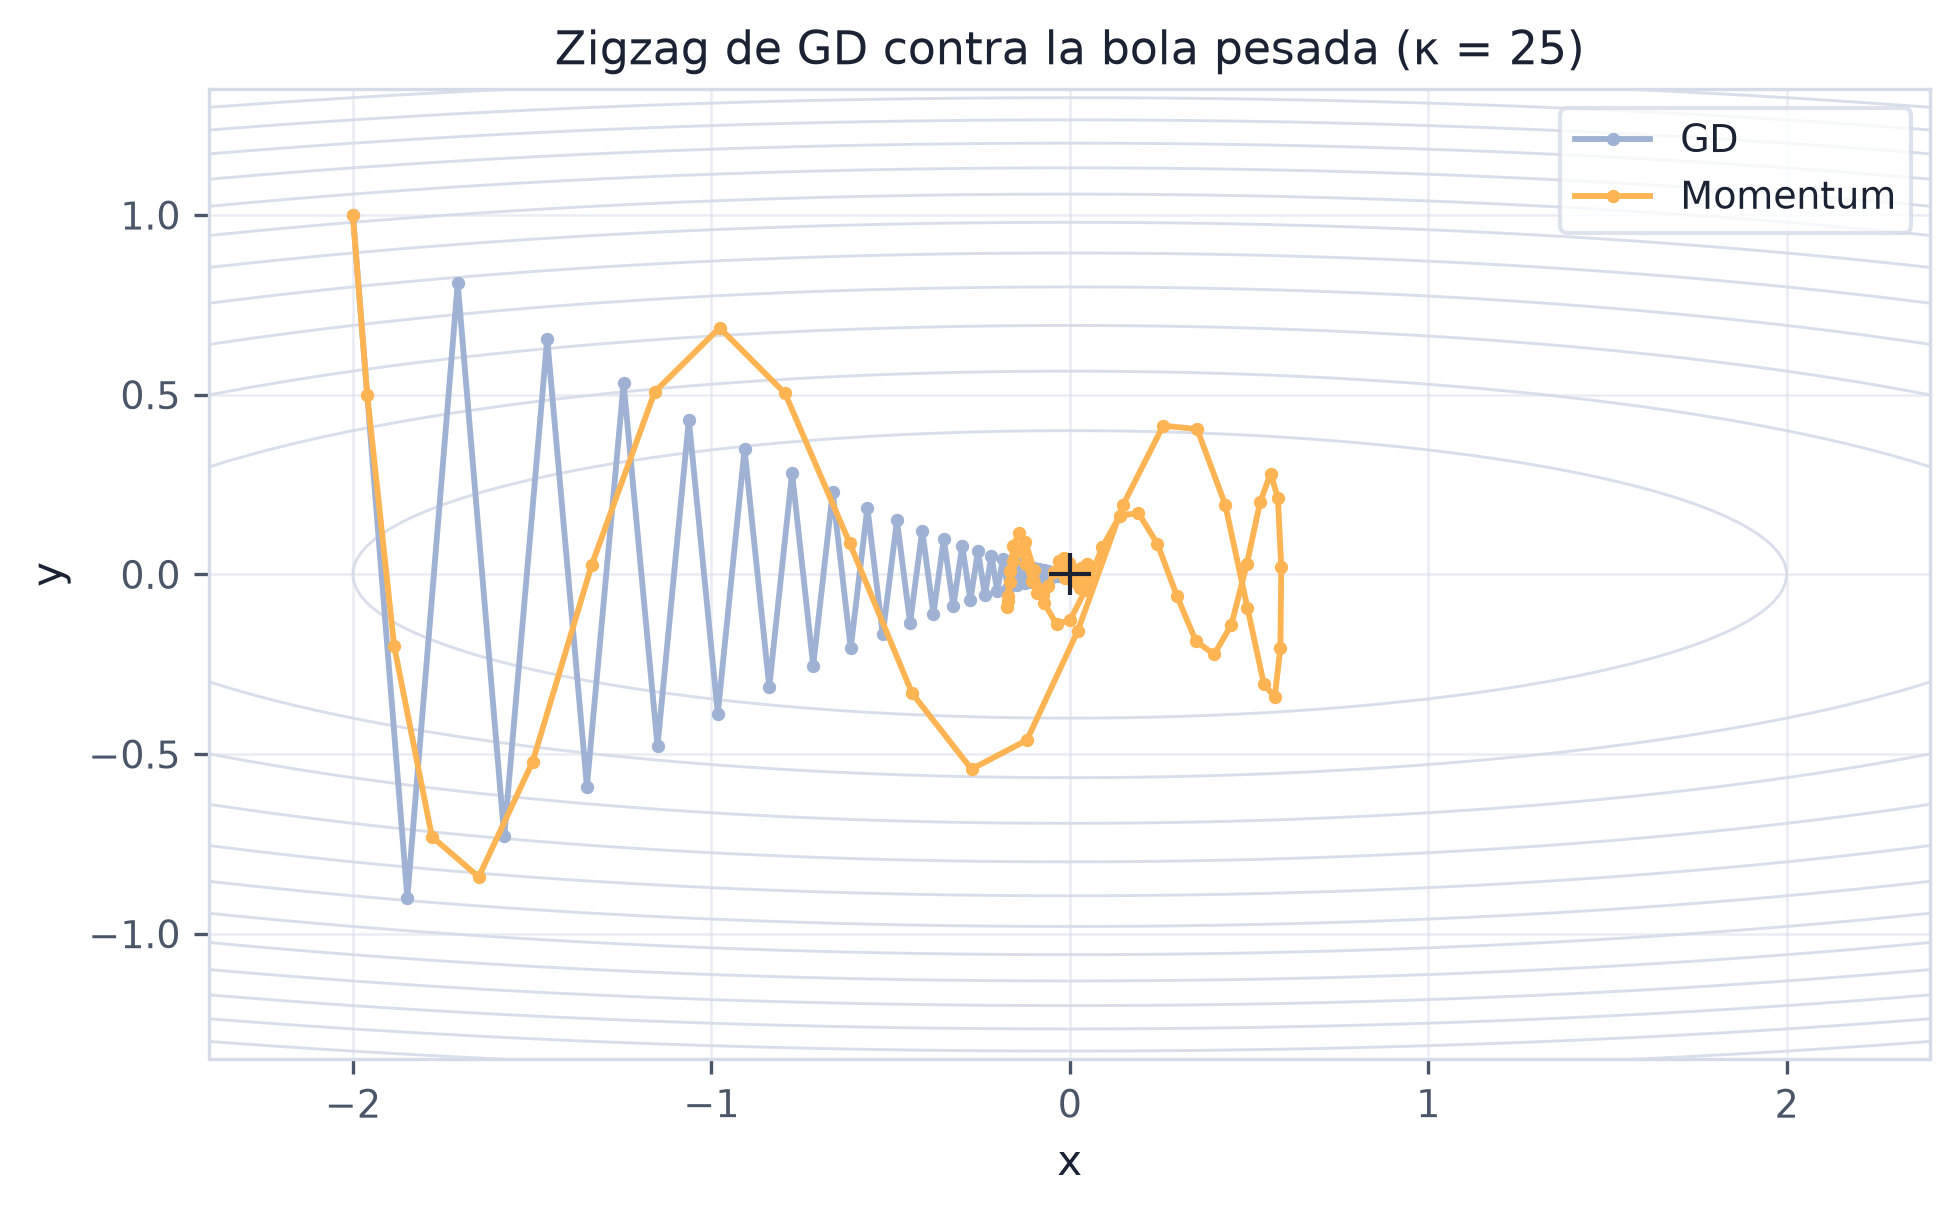
\includegraphics[width=\columnwidth]{fig-ravine-light.png}
  \caption{GD ($\alpha = 0.076$, 90 iteraciones) y Momentum ($\alpha = 0.02$, $\beta = 0.9$, 150 iteraciones) sobre la cuadrática $f(x,y) = \frac{1}{2}(x^2 + 25y^2)$, desde $(-2, 1)$.}
  \label{fig:ravine}
\end{figure}

La Fig.~\ref{fig:ravine} muestra el valle cuadrático con $\kappa = 25$. Para avanzar en la dirección blanda, GD necesita operar cerca de su límite de estabilidad~\eqref{eq:estabilidad}, que aquí es $2/25 = 0.08$: con $\alpha = 0.076$, el $95\,\%$ del límite, el factor de error en la dirección rígida es casi $-1$ y la trayectoria rebota de pared a pared, el zigzag clásico. Tras 90 iteraciones termina en $f \approx 1.4 \times 10^{-6}$. Momentum, con una tasa cuatro veces menor ($\alpha = 0.02$, $\beta = 0.9$), amortigua la componente alternante y rueda por el fondo del valle: alcanza $f \approx 6.3 \times 10^{-8}$ en 150 iteraciones con una trayectoria visiblemente limpia. La geometría que a GD le cobra el zigzag es exactamente la que Momentum repara, como predice la mejora de $\kappa$ a $\sqrt{\kappa}$ de la Sección~\ref{sec:momentum}.

\subsection{La carrera sobre Rosenbrock}

\begin{figure}[t]
  \centering
  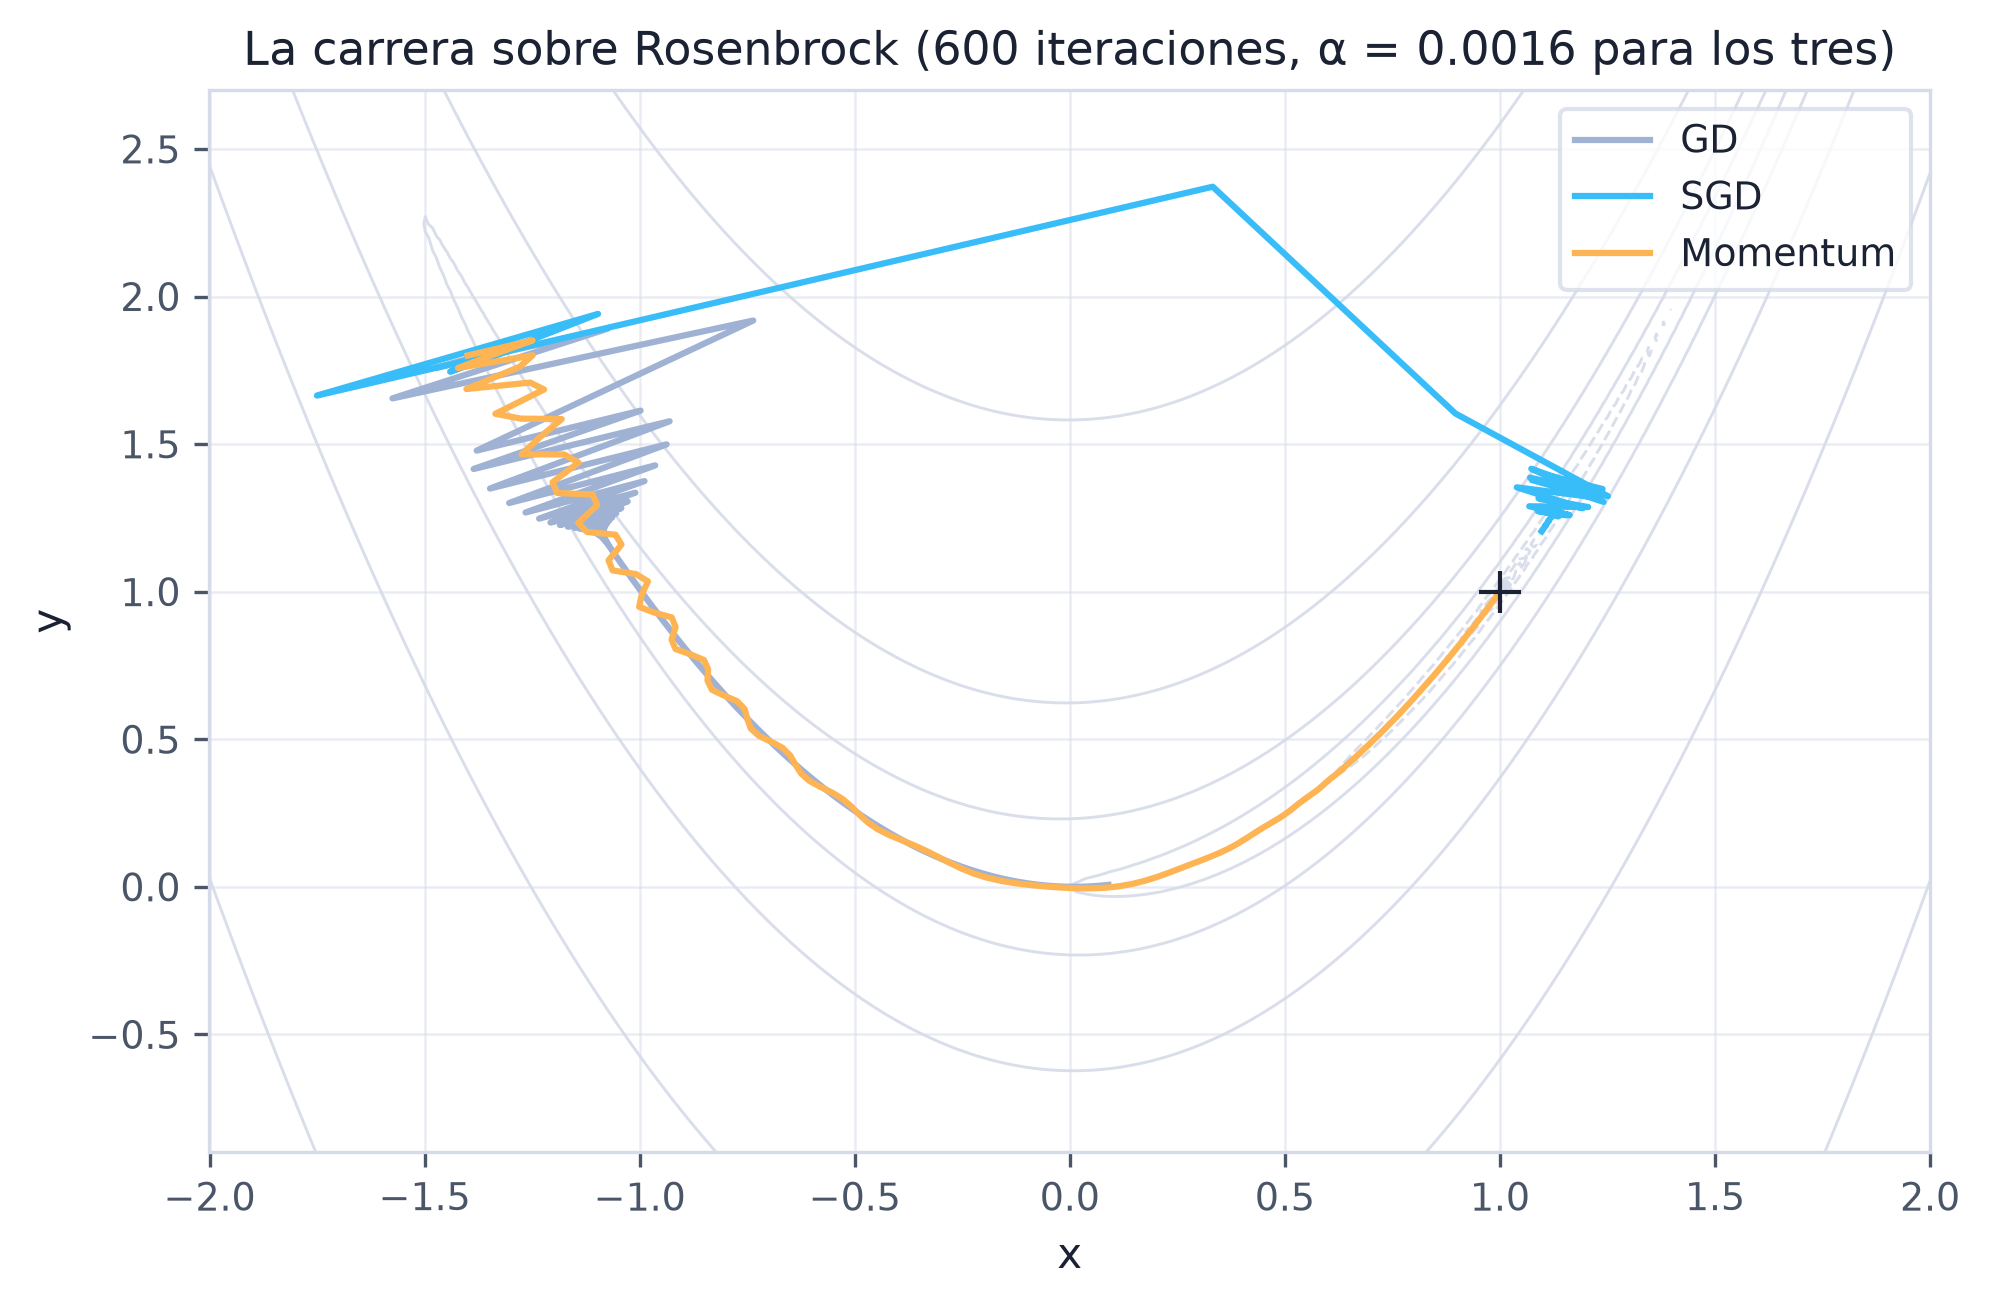
\includegraphics[width=\columnwidth]{fig-rosenbrock-light.png}
  \caption{Los tres métodos sobre Rosenbrock con la misma $\alpha = 0.0016$ y 600 iteraciones, desde $(-1.4, 1.8)$. Las curvas de nivel están en escala logarítmica. GD termina en $f \approx 0.83$, la variante con ruido inyectado en $f \approx 9.5 \times 10^{-3}$ (véase el texto) y Momentum en $f \approx 4.7 \times 10^{-5}$, prácticamente en el mínimo $(1,1)$.}
  \label{fig:rosen}
\end{figure}

La función de Rosenbrock, $f(x,y) = (1-x)^2 + 100\,(y - x^2)^2$, con mínimo único en $(1,1)$, es el banco de pruebas clásico: su valle es fácil de encontrar y difícil de recorrer, porque el piso es casi plano y se curva, mientras que las paredes parabólicas son empinadas. Las paredes atan las manos con la tasa: un $\alpha$ lo bastante grande para avanzar de verdad por el piso sale catapultado, así que debe ser diminuto, $\alpha = 0.0016$. La Fig.~\ref{fig:rosen} muestra la carrera: los tres métodos con la misma $\alpha$ y 600 iteraciones desde $(-1.4, 1.8)$.

GD baja al valle de inmediato y luego se arrastra. Sin memoria, su avance por iteración es $\alpha$ por el gradiente actual, y el gradiente del piso es diminuto: termina en $f \approx 0.83$, todavía lejos del mínimo. Momentum acumula los gradientes del piso, que apuntan consistentemente a lo largo del valle, conserva la velocidad en la curva y llega prácticamente al mínimo: $f \approx 4.7 \times 10^{-5}$, cuatro órdenes de magnitud por debajo de GD con el mismo presupuesto. El terreno plano y curvo es exactamente donde la memoria paga: ahí avanzar es cuestión de distancia acumulada, y el único que acumula es Momentum.

La curva etiquetada SGD merece una aclaración de honestidad experimental. Sobre una función de prueba pura no hay datos que muestrear, así que el estimador estocástico se simula inyectando al gradiente exacto un ruido gaussiano proporcional a su norma ($15\,\%$, semilla fija). En las paredes, donde el gradiente es enorme, el ruido también lo es, y con la semilla de la figura una de esas sacudidas lanza el iterado por encima del tazón hasta la otra rama del valle, donde queda temblando alrededor de $f \approx 9.5 \times 10^{-3}$ sin asentarse. Ese salto es suerte de la semilla, no una propiedad del método: en corridas con cinco semillas distintas el mismo esquema termina entre $f \approx 0.67$ y $f \approx 1.3$, comparable o peor que GD. La lección es doble: el ruido sin estructura no aporta información en una función pura (el valor de SGD vive en las sumas sobre datos), y el contraste que sí es estable entre corridas es el de GD contra Momentum, porque ambos son deterministas.

\subsection{Regresión logística sobre datos reales}

\begin{figure}[t]
  \centering
  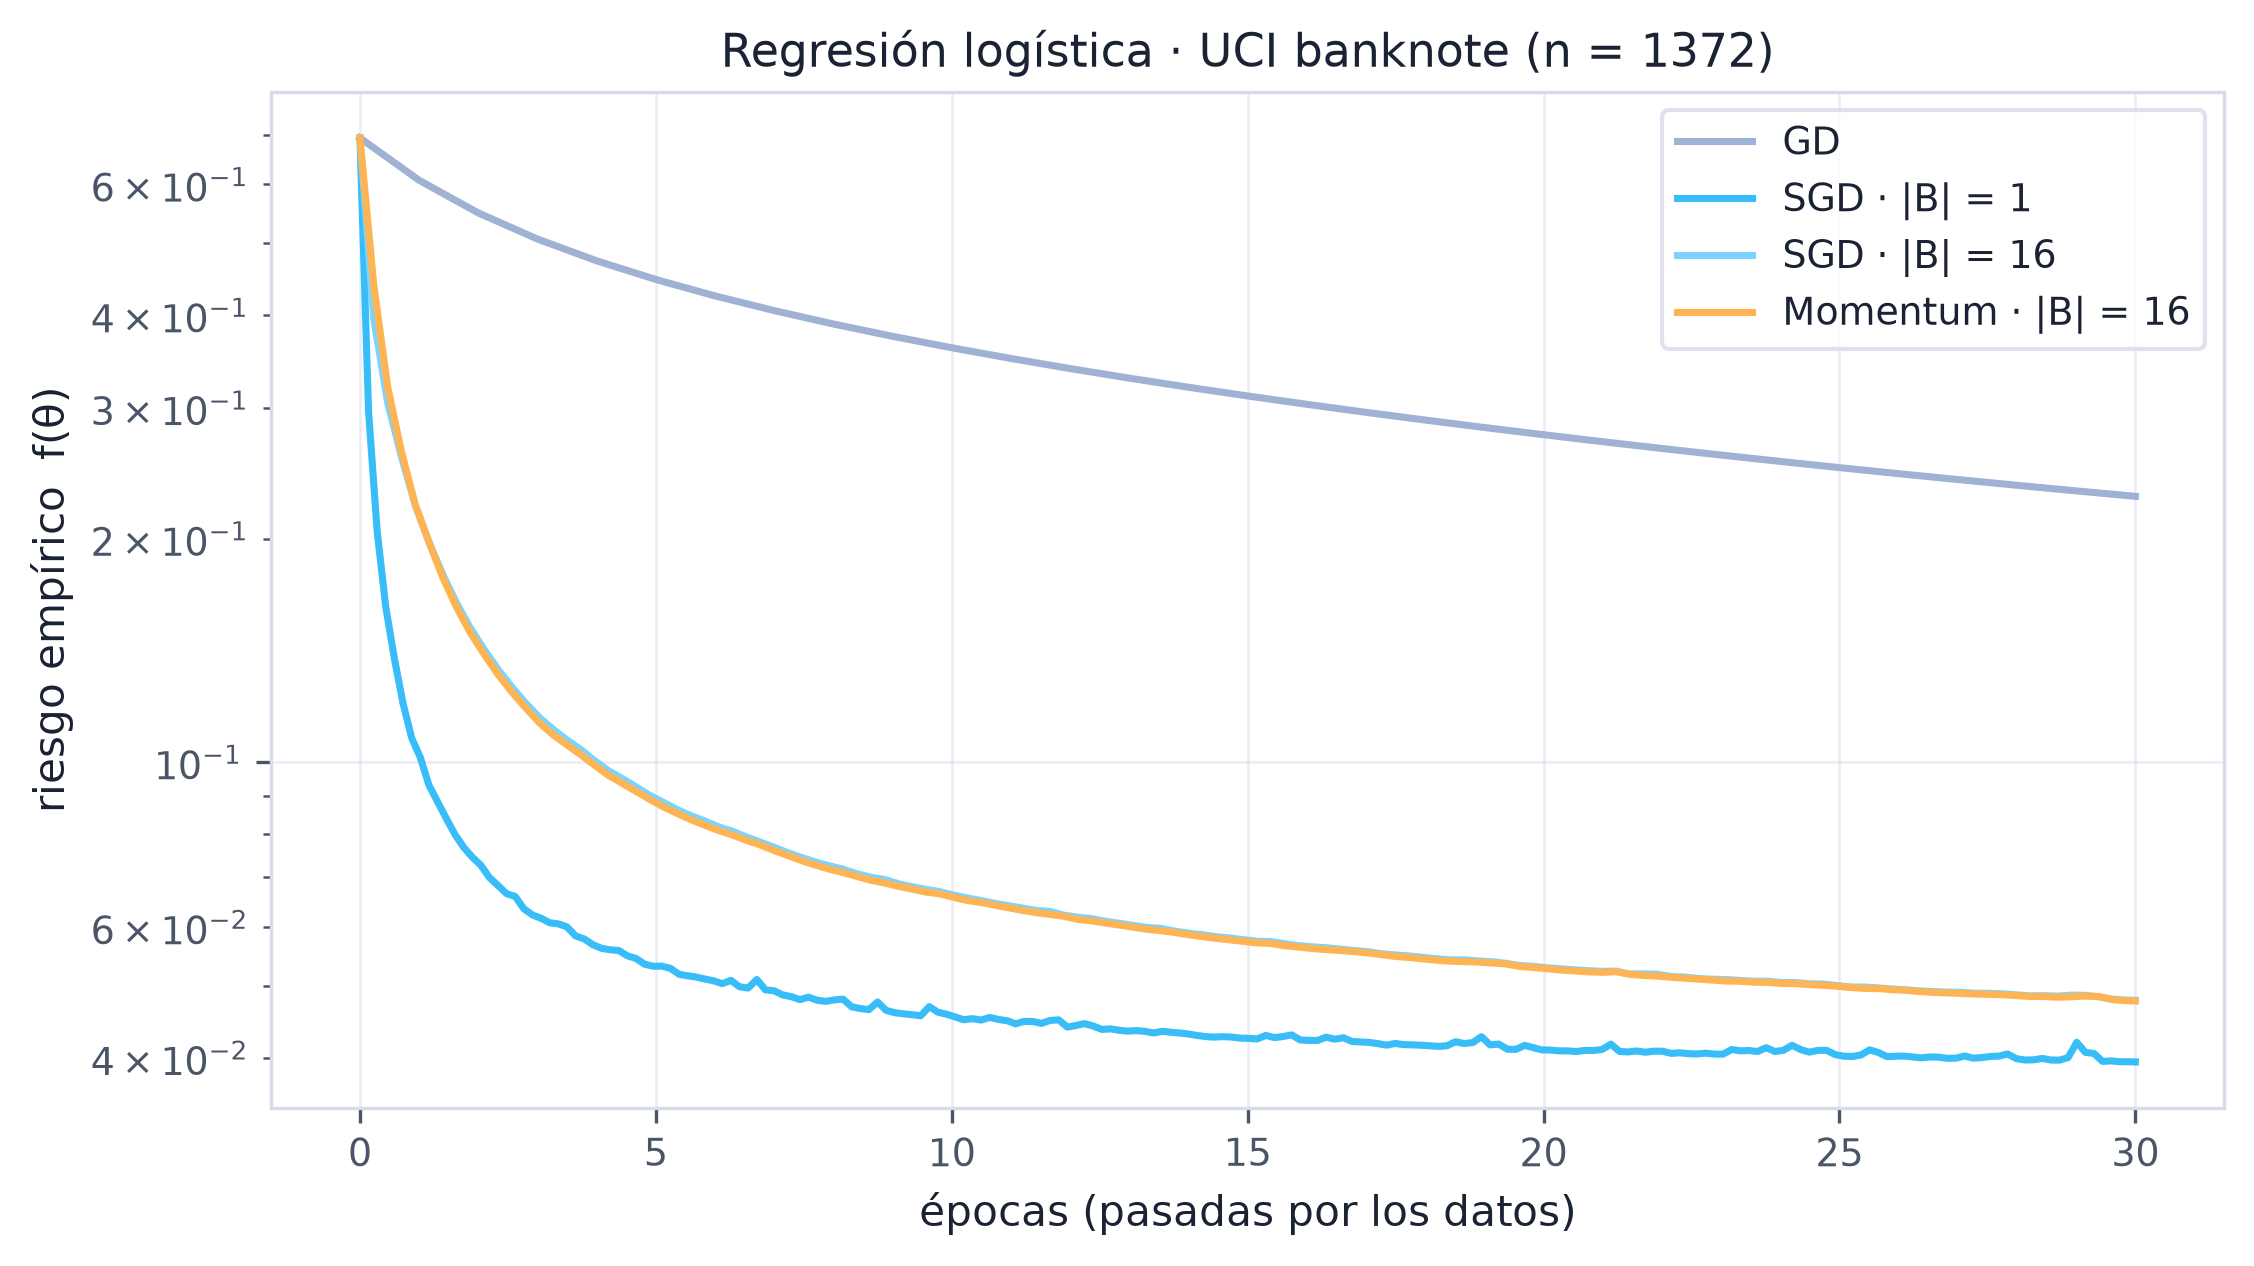
\includegraphics[width=\columnwidth]{fig-logistic-light.png}
  \caption{Riesgo empírico contra épocas en la regresión logística regularizada sobre banknote ($n = 1372$), con presupuesto de 30 épocas: GD ($\alpha = 0.5$), SGD con $|B| = 1$ ($\alpha = 0.05$), SGD con $|B| = 16$ ($\alpha = 0.2$) y Momentum con $|B| = 16$ ($\alpha = 0.02$, $\beta = 0.9$).}
  \label{fig:logistic}
\end{figure}

\begin{table}[t]
  \caption{Exactitud de clasificación al final de las corridas de la Fig.~\ref{fig:logistic}, sobre el conjunto completo ($n = 1372$).}
  \label{tab:acc}
  \centering
  \begin{tabular}{lccc}
    \toprule
    Método & $\alpha$ & $|B|$ & Exactitud \\
    \midrule
    GD & 0.5 & $n$ & 0.9453 \\
    SGD & 0.05 & 1 & 0.9905 \\
    SGD & 0.2 & 16 & 0.9818 \\
    Momentum ($\beta = 0.9$) & 0.02 & 16 & 0.9818 \\
    \bottomrule
  \end{tabular}
\end{table}

El experimento central usa el conjunto UCI Banknote Authentication~\cite{lohweg2013}: 1372 billetes, cada uno con cuatro características extraídas de su imagen mediante wavelets y una etiqueta de genuino o falso. Se entrena una regresión logística con penalización $\ell_2$ pequeña ($\lambda = 10^{-4}$) sobre los rasgos estandarizados más un sesgo, cinco parámetros en total. La pérdida logística es convexa y la penalización la vuelve fuertemente convexa: hay un único mínimo global, y las garantías de las secciones anteriores aplican.

La Fig.~\ref{fig:logistic} compara los métodos con el eje horizontal en épocas, la comparación honesta de la Sección~\ref{sec:sgd}. Tres lecturas. Primero, los métodos estocásticos dominan a GD desde la primera pasada: GD realiza una iteración por época, apenas 30 actualizaciones en todo el presupuesto, mientras que SGD con $|B| = 1$ realiza 1372 iteraciones por época, unas $41\,000$ en total. Segundo, la curva de $|B| = 16$ es visiblemente más limpia que la de $|B| = 1$, como predice la varianza proporcional a $1/|B|$ de la Sección~\ref{sec:minilotes}, sin perder velocidad por época y tolerando además una tasa cuatro veces mayor. Tercero, Momentum no aporta aquí: con los rasgos estandarizados el problema queda bien acondicionado y no hay cañón que reparar, así que su curva es comparable a la de SGD con el mismo lote. Es el contraste honesto con Rosenbrock: la ventaja de Momentum es geométrica, no universal.

La Tabla~\ref{tab:acc} resume la exactitud de clasificación al final de cada corrida. Dos advertencias de lectura: el experimento no separa un conjunto de prueba, así que las cifras miden ajuste sobre los mismos datos, no generalización; y la diferencia entre las tres variantes estocásticas (alrededor de un punto porcentual) es del orden del ruido de una corrida individual y no debe sobreinterpretarse. La lectura robusta es la brecha grande: dentro del mismo presupuesto de 30 épocas, cualquiera de las variantes estocásticas resuelve el problema mientras que GD queda lejos de converger.

\subsection{Sensibilidad a la tasa de aprendizaje}

\begin{figure}[t]
  \centering
  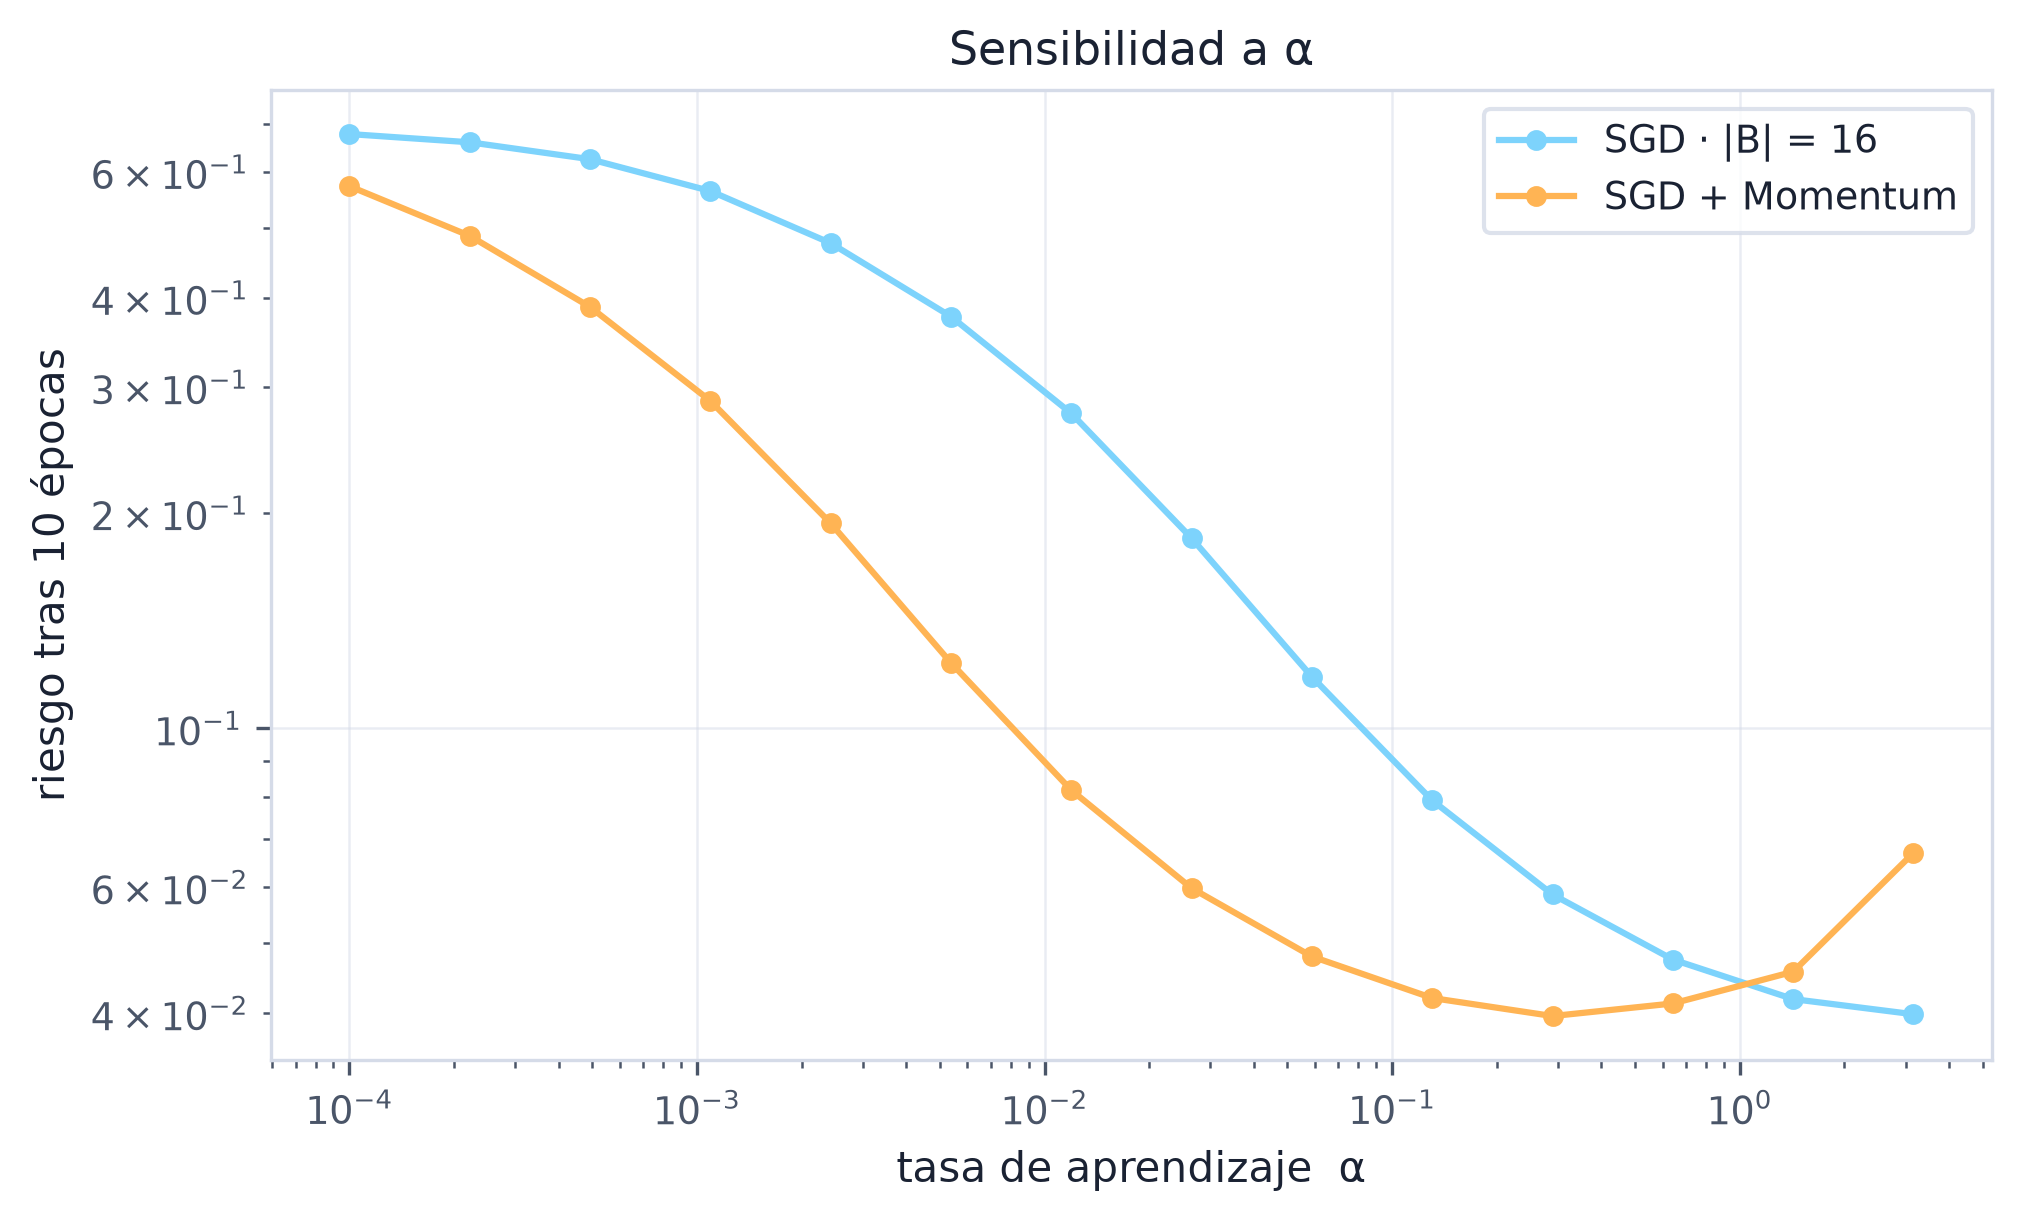
\includegraphics[width=\columnwidth]{fig-lr-sensitivity-light.png}
  \caption{Riesgo tras 10 épocas sobre banknote, para 14 valores de $\alpha$ entre $10^{-4}$ y $10^{0.5}$, con $|B| = 16$: SGD y SGD con Momentum ($\beta = 0.9$). Ambos ejes en escala logarítmica.}
  \label{fig:lr}
\end{figure}

La Fig.~\ref{fig:lr} barre la tasa de aprendizaje sobre el mismo problema y deja dos lecturas. Primero, la forma general de ambas curvas: una meseta amplia de valores útiles con deterioro hacia los extremos. Elegir $\alpha$ no exige precisión de laboratorio, pero equivocarse por órdenes de magnitud sí cuesta. Segundo, la curva de Momentum es, a grandes rasgos, la de SGD desplazada una década hacia la izquierda: como la velocidad se compone hacia $g/(1-\beta) = 10\,g$ con $\beta = 0.9$, el paso efectivo se amplifica por diez. Momentum alcanza su mejor riesgo cerca de $\alpha \approx 0.3$ y se degrada pasado $\alpha \approx 1$, donde SGD solo todavía mejora. En este problema bien acondicionado ambos alcanzan mínimos comparables, alrededor de $4 \times 10^{-2}$: Momentum no llega más abajo, llega con una tasa diez veces menor, en línea con la subsección anterior.

\subsection{Parada temprana}

\begin{figure}[t]
  \centering
  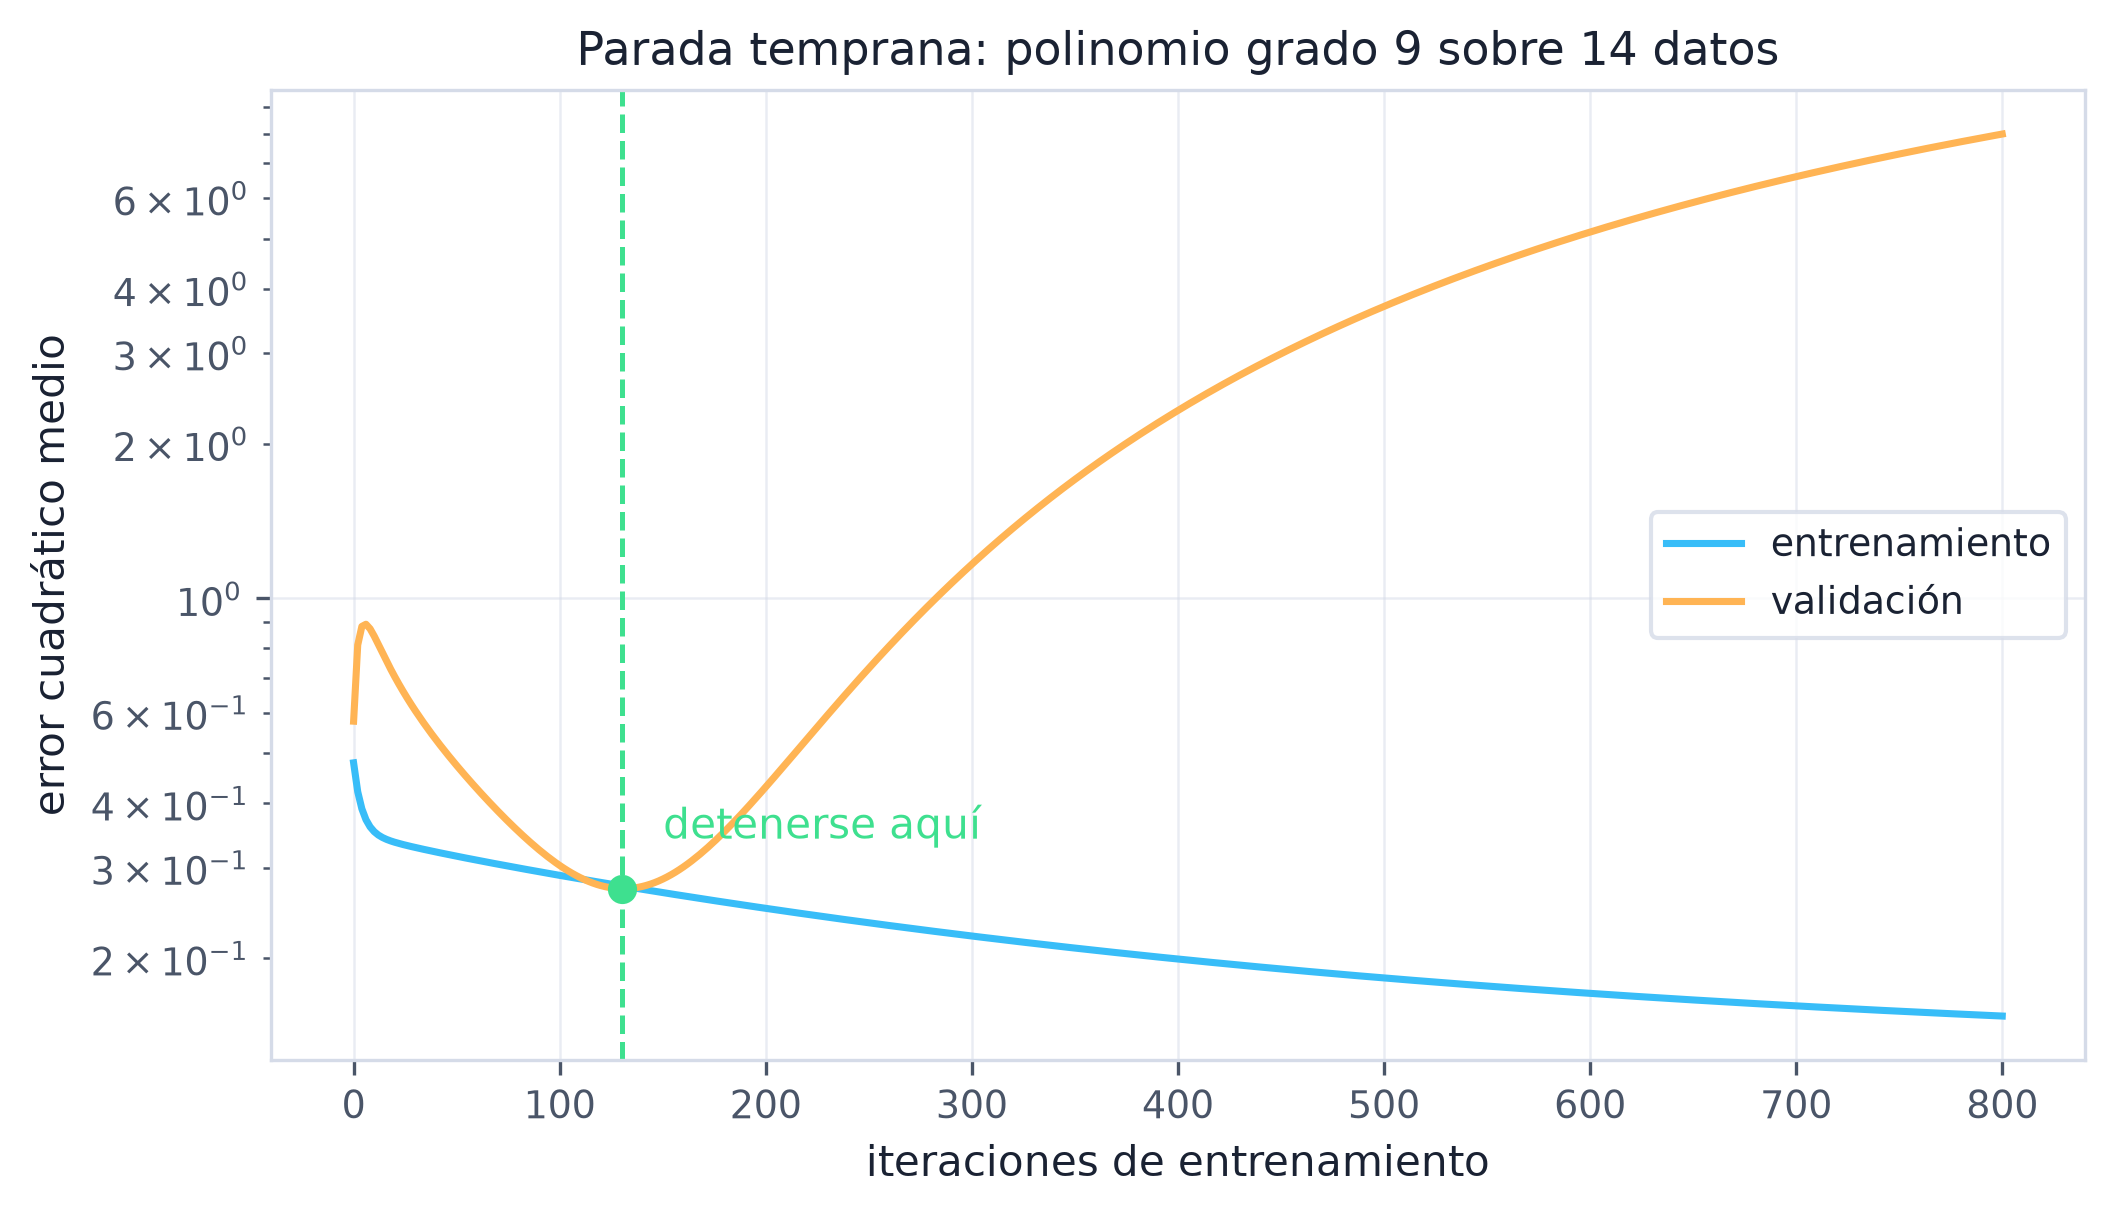
\includegraphics[width=\columnwidth]{fig-early-stopping-light.png}
  \caption{Errores de entrenamiento y validación para un polinomio de grado 9 ajustado por GD ($\alpha = 0.06$) a 14 datos, con 20 datos de validación. El mínimo de validación ocurre en la iteración 130 de 800.}
  \label{fig:early}
\end{figure}

El último experimento aísla la parada temprana con un modelo de capacidad sobrada: un polinomio de grado 9 (diez coeficientes) ajustado a solo 14 datos de entrenamiento, con 20 datos de validación apartados, por GD de lote completo durante 800 iteraciones. La Fig.~\ref{fig:early} muestra el patrón que la Sección~\ref{sec:minilotes} anticipa. El error de entrenamiento baja de forma monótona durante toda la corrida. El de validación baja, toca su mínimo en la iteración 130 y vuelve a subir sin pausa: al final de la corrida es 29 veces su mínimo. Detenerse en ese mínimo captura la señal sin el sobreajuste. Es la regularización gratuita en su forma más pura: ningún término extra en la función objetivo, solo la decisión de mirar el error correcto, el de validación, y parar a tiempo.

\section{Conclusiones}\label{sec:concl}

Cuatro conclusiones, cada una respaldada por un experimento de la Sección~\ref{sec:exp}.

\emph{El trato de SGD gana a escala.} Sustituir el gradiente exacto por un estimador insesgado cambia precisión por costo en cada iteración, y el presupuesto rinde más: sobre banknote, los métodos estocásticos dominan a GD desde la primera época y resuelven el problema dentro de un presupuesto en el que GD ni siquiera se acerca a converger. La insesgadez~\eqref{eq:insesgado} garantiza que el ahorro no se paga con sesgo, solo con ruido.

\emph{El lote es la perilla de la varianza.} El promedio de mini-lote~\eqref{eq:minibatch} conserva la insesgadez, reduce la varianza del ruido como $1/|B|$ y mantiene constante el costo por época. En los datos reales, $|B| = 16$ produce una curva visiblemente más limpia que $|B| = 1$ y tolera una tasa mayor, sin perder velocidad por época. En la práctica, el lote se elige tan grande como la memoria permita.

\emph{La parada temprana es regularización sin costo.} El mínimo del error de validación llega mucho antes que el final del entrenamiento (la iteración 130 de 800 en el experimento) y pasarlo de largo multiplica ese error por casi treinta. Detenerse ahí equivale a una penalización $\ell_2$ implícita y solo requiere monitorear el error correcto.

\emph{Momentum repara la geometría.} Donde el condicionamiento es adverso, la memoria de gradientes cancela el zigzag y compone el avance persistente: cuatro órdenes de magnitud por debajo de GD en Rosenbrock, con la misma tasa y el mismo número de iteraciones. Donde el problema ya está bien acondicionado, como en banknote con rasgos estandarizados, no aporta. Su ventaja es geométrica, no universal, y saber cuándo una herramienta no ayuda es parte de entenderla.

En una frase: entrenar es minimizar un promedio sobre datos, y la eficiencia sale de estimar el gradiente barato, dosificar su varianza con el lote, detenerse a tiempo y corregir la geometría con memoria.


\bibliographystyle{IEEEtran}
\bibliography{references}

\end{document}
